\documentclass[12pt]{article}
\usepackage{amsmath}
\usepackage{amssymb}
\usepackage{amsthm}
\usepackage{amsfonts}
\usepackage{graphicx}
\usepackage{textcomp}
\usepackage{hyperref}
\usepackage{tikz}
\usepackage{enumitem}
\usepackage{mathtools}
\usepackage{float}
\usepackage{cleveref}
\usepackage{hyperref}
\usepackage{csquotes}

\begin{document}

\title{MACM 101 Chapter 1.3 - Logical Identities}
\author{Alexander Ng}
\date{Sunday, September 15, 2024}

\maketitle

This document covers Rosen 1.3, Pearce 1.1 72-xx.

\section*{Summary}

\begin{enumerate}
\item Tautologies, Contradictions and Contingencies
\item Logical Equivalence
  \subitem Important Logical Equivalences
  \subitem Showing Logical Equivalences
\item Logical Implication (not in Rosen)
\item Normal Forms
  \subitem Distributive Normal Form (DNF)
  \subitem Conjunctive Normal Form (CNF)
\end{enumerate}

% reminder to self: add refs to each section

\pagebreak

\section{Tautologies, Contradictions and Contingencies}

\noindent

A Tautology (\textbf{T}) is a proposition that is always true.

\textbf{Example:} $p \lor \neg p$

A Contradiction (\textbf{F}) is a proposition that is always false.

\textbf{Example:} $p \land \neg p$

A contingency is a proposition that is neither a tautology nor a contradiction,
such as $p$.

\section{Logical Equivalences}

Two statements, $s_1$ and $s_2$ are said to be logically equivalent if, when one
is true, the other is also true, and conversely, when one is false, the other
is also false.

In other words, two statements are logically equivalent if they have identical
truth tables.

\begin{itemize}
\item We write $s_1 \Leftrightarrow s_2$ to denote that $s_1$ and $s_2$ are
  logically equivalent.
\item Conversely, we write $s_1 \nLeftrightarrow s_2$ to denote that $s_1$
  and $s_2$ are not logically equivalent.
\item The symbol $\equiv$ is also used to denote logical equivalence.
\end{itemize}


\subsection{Implication and it's Cousins}

\[
\begin{array}{|c|c|c|c|c|c|}
\hline
p & q & p \to q & q \to p & \neg p \to \neg q & \neg q \to \neg p \\
\hline
0 & 0 & 1 & 1 & 1 & 1 \\
0 & 1 & 1 & 0 & 0 & 1 \\
1 & 0 & 0 & 1 & 1 & 0 \\
1 & 1 & 1 & 1 & 1 & 1 \\
\hline
\end{array}
\]

Clearly, $p \to q \Leftrightarrow \neg q \to \neg p$ and 
$q \to p \Leftrightarrow \neg p \to \neg q$.

\begin{itemize}
\item $p \to q$ is called \textbf{material implication}
\item $q \to p$ is called the \textbf{converse} of material implication
\item $\neg q \to \neg p$ is called the \textbf{contrapositive} of material
  implication
\item $\neg p \to \neg q$ is called the \textbf{inverse} of material
  implication
\end{itemize}

\subsection{The Formal Axiomatic System of Propositional Logic}

Logical equivalence is the foundation of the formal axiomatic system of
propositional logic.

The goal of this aximoatic system, and the following propositional identities,
is to provide an algebraic foundation for simplifying expressions.

\subsection{Propositional Identities}

\subsubsection{Identity 1 - Implication Reduction}

\begin{equation}
  p \to q \equiv \neg p \lor q
  \label{eq:identity_1}
\end{equation}

\[
\begin{array}{|c|c|c|c|}
\hline
p & q & p \to q & \neg p \lor q \\
\hline
0 & 0 & 1 & 1 \\
0 & 1 & 1 & 1 \\
1 & 0 & 0 & 0 \\
1 & 1 & 1 & 1 \\
\hline
\end{array}
\]

\begin{itemize}
\item $p \to q$ means $p \therefore q$
\item If the argument is valid and $p$ is true, then $q$ is also true.
\item If the argument is valid and $p$ is false, then we can conclude nothing
  about $q$.
\item Thus, $p \to q$ is logically equivalent to $\neg p \lor q$
\end{itemize}

**Implication Reduction will be one of the most important identities in
propositional logic.

\subsubsection{Identity 2 - De Morgan's Laws}

\begin{align}
  \neg (p \land q) &\equiv \neg p \lor \neg q \\
  \neg (p \lor q) &\equiv \neg p \land \neg q
\end{align}

We can prove De Morgan's laws by using a truth table.

\begin{figure}[H]
    \centering
    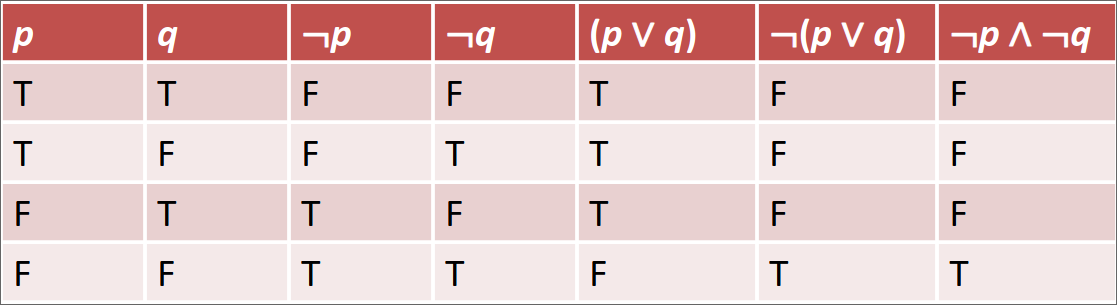
\includegraphics[width=0.8\textwidth]{"./de_morgans_second_law.png"}
    \caption{De Morgan's Second Law}
\end{figure}

Breaking down the truth table, column by column, we can see that De Morgan's
laws do indeed hold. These will become fundamental for the algebraic
manipulation of propositions.

\begin{figure}[H]
    \centering
    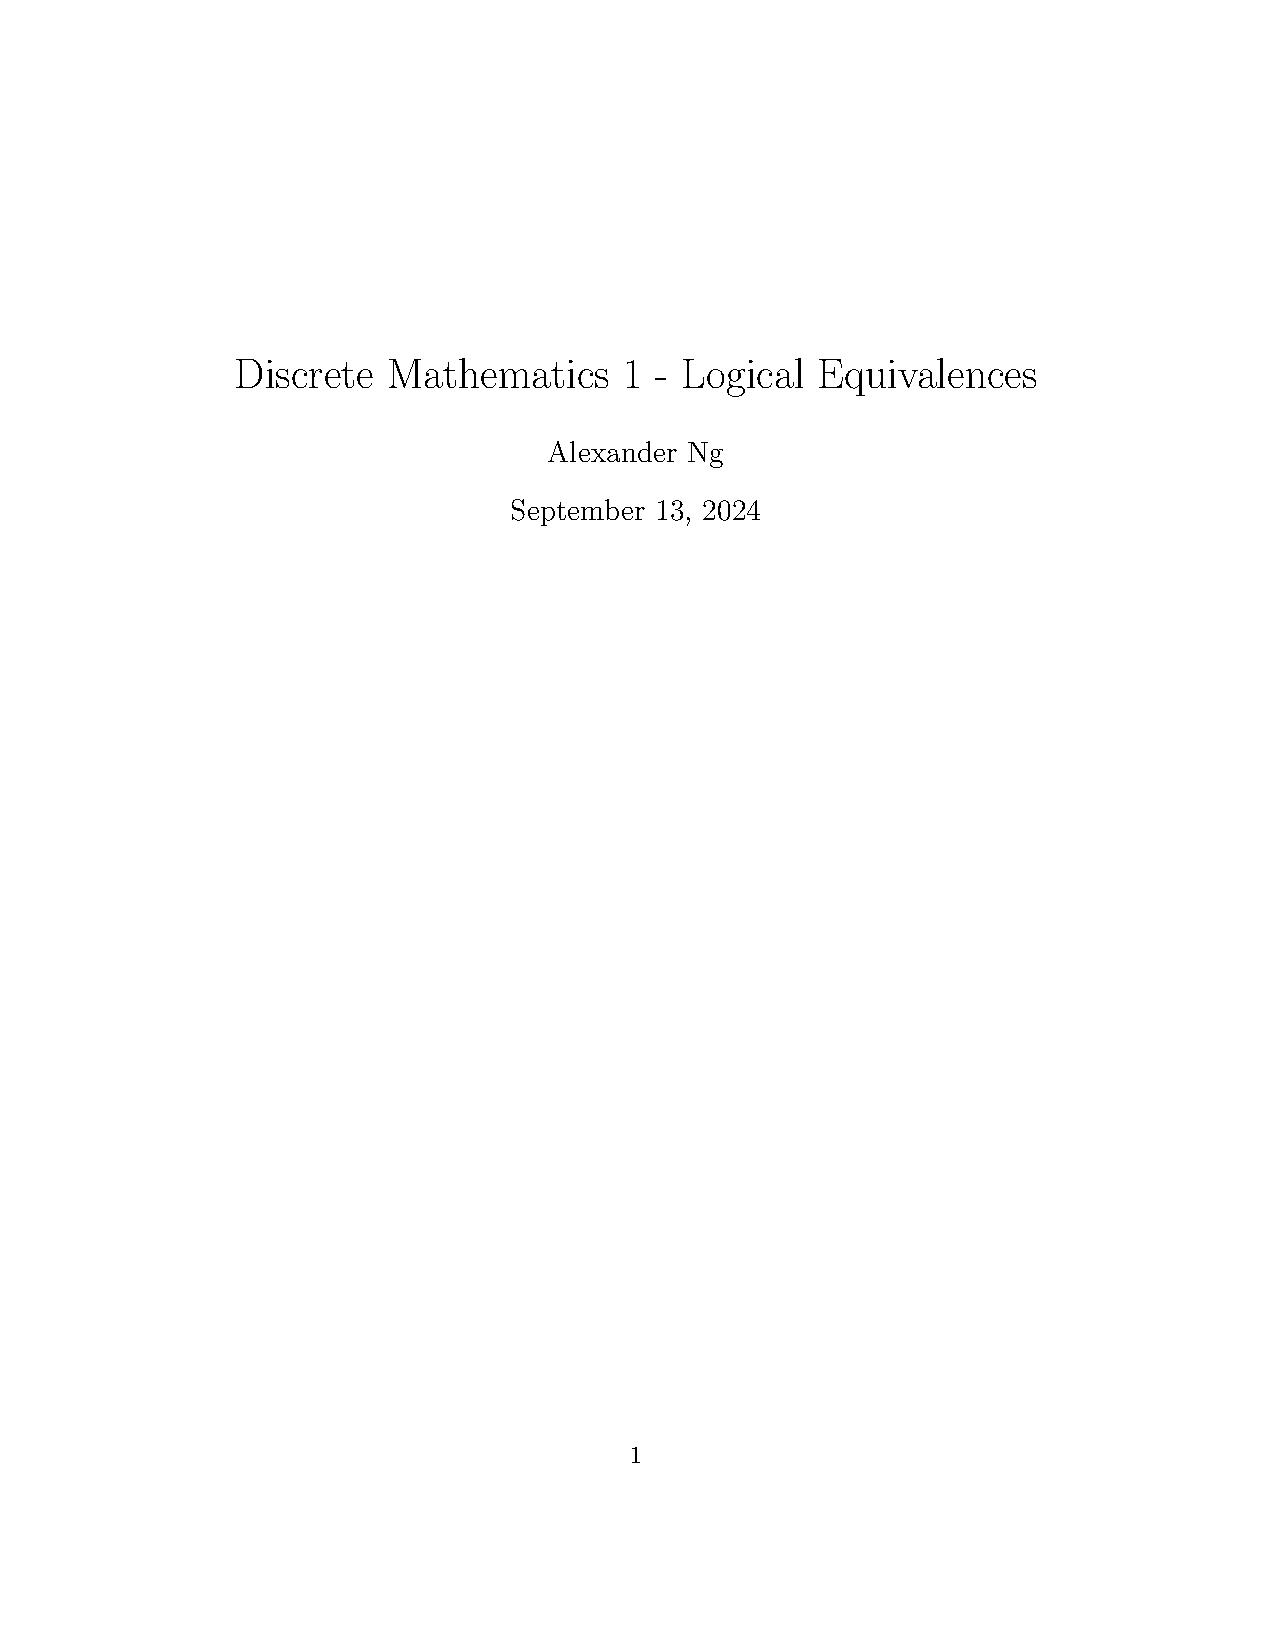
\includegraphics[width=0.8\textwidth]{"./Logical Equivalences.jpg"}
    \caption{Logical Equivalences}
\end{figure}

\begin{figure}[H]
    \centering
    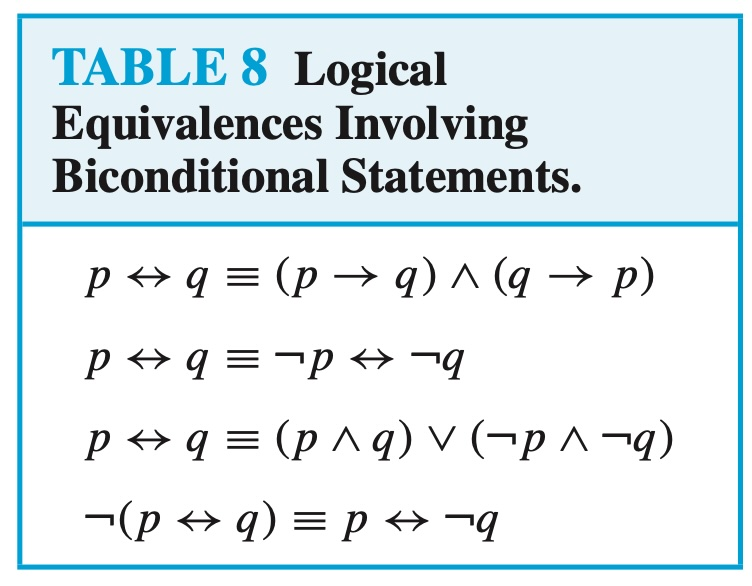
\includegraphics[width=0.4\textwidth]{"./Logical Equivalences Involving Biconditional Statements.jpg"}
    \caption{Logical Equivalences Involving Biconditional Statements}
\end{figure}

\begin{figure}[H]
    \centering
    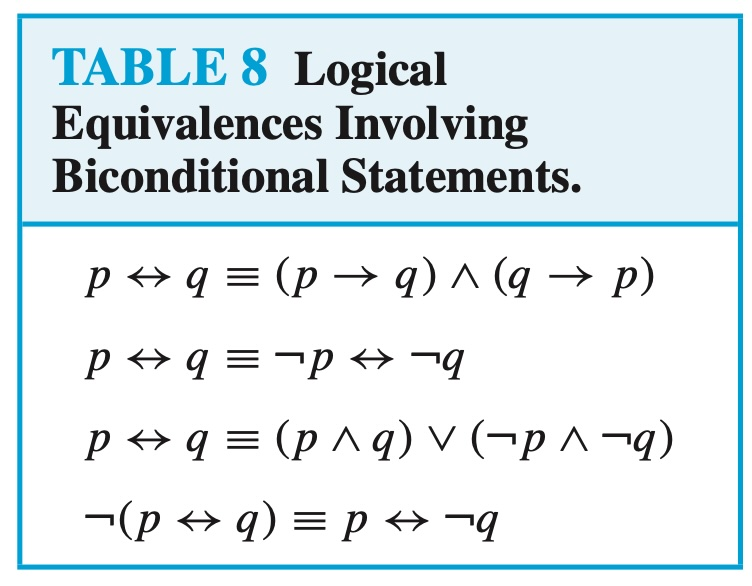
\includegraphics[width=0.4\textwidth]{"./Logical Equivalences Involving Biconditional Statements.jpg"}
    \caption{Logical Equivalences Involving Conditional Statements}
\end{figure}

\end{document}
